\documentclass[10pt, letterpaper]{report}
% !TeX program = xelatex
%==================PREAMBOLO=======================%
\usepackage[utf8]{inputenc}
\usepackage{psvectorian}
\usepackage{pgfplots}
\usepackage[Rejne]{fncychap}
\usepackage[export]{adjustbox}
\usepackage[T1]{fontenc}
\usepackage{lmodern}
\usepackage[shortlabels]{enumitem}
\usepackage{moresize}
\usepackage{graphicx} % Required for inserting images
\usepackage{hyperref}
\usepackage{listings}
\usepackage[table,xcdraw]{xcolor}
\usepackage{amssymb}
\usepackage{amsmath}
\usepackage[italian]{babel}
\usepackage{nicefrac, xfrac}
\usepackage{tikz}
\usepackage{mathrsfs} 
\usepackage{titletoc}
\usepackage{fancyhdr}
\usepackage{psvectorian,lipsum}
\usepackage{fourier-orns}
\usepackage{lipsum}
\usepackage[paper=a4paper,left=25mm,right=25mm,bottom=25mm,top=25mm]{geometry}
\definecolor{light-gray}{gray}{0.95}
\definecolor{cop}{HTML}{f7ecd7}
\definecolor{copAut}{HTML}{ababab}
\definecolor{copAut2}{HTML}{c3c3e6}
\definecolor{purcop}{HTML}{d0d3db}
\definecolor{sapienza}{HTML}{660f1d}
\definecolor{lightSapienza}{HTML}{e3d3d5}
\definecolor{darkgreen}{HTML}{008000}
\definecolor{cartaRiciclata}{HTML}{fcfcf7}
\newcommand{\redText}[1]{\color{red}#1\color{black}}
\newcommand{\code}[1]{\colorbox{light-gray}{\texttt{#1}}}
\newcommand{\codee}[1]{\colorbox{white}{\texttt{#1}}}
\newcommand{\K}{{\mathbb K}}
\newcommand{\notimplies}{%
  \mathrel{{\ooalign{\hidewidth$\not\phantom{=}$\hidewidth\cr$\implies$}}}}
\newcommand{\flowerLine}{ \begin{center}\decofourleft\hphantom{ }\decoone\hphantom{ }\decofourright\hphantom{}\hphantom{aa}
\decofourleft\hphantom{ }\decoone\hphantom{ }\decofourright\hphantom{}\hphantom{aa}
\decofourleft\hphantom{ }\decoone\hphantom{ }\decofourright\hphantom{}\hphantom{aa}
\decofourleft\hphantom{ }\decoone\hphantom{ }\decofourright\hphantom{}\hphantom{aa} 
\decofourleft\hphantom{ }\decoone\hphantom{ }\decofourright\hphantom{}\hphantom{aa}
\decofourleft\hphantom{ }\decoone\hphantom{ }\decofourright\hphantom{}\hphantom{aa}
\decofourleft\hphantom{ }\decoone\hphantom{ }\decofourright\hphantom{}\hphantom{aa}
\decofourleft\hphantom{ }\decoone\hphantom{ }\decofourright\hphantom{}\hphantom{aa}
\decofourleft\hphantom{ }\decoone\hphantom{ }\decofourright\hphantom{}\hphantom{aa}
\end{center}}
\definecolor{g}{RGB}{60, 50, 50}
\newcommand{\textg}[1]{\color{g}{\textbf{#1}}\color{black}}
\newcommand{\teo}[1]{{\large\color{sapienza}\textbf{Teorema #1 :\hphantom{a}}}}
\newcommand{\defi}[1]{{\large\color{sapienza}\textbf{Definizione #1 :\hphantom{a}}}}
\newcommand{\claim}[1]{{\color{sapienza}\textbf{Claim #1 :\hphantom{a}}}}
\newcommand{\lemma}[1]{{\color{sapienza}\textbf{Lemma #1 :\hphantom{a}}}}
\newcommand{\dimo}[1]{{\color{sapienza}\textbf{Dimostrazione #1 :\hphantom{a}}}}
\newcommand{\prop}[1]{{\color{sapienza}\textbf{Proposizione #1 :\hphantom{a}}}}
\newcommand\greybox[1]{%
  \vskip\baselineskip%
  \par\noindent\colorbox{light-gray}{%
    \begin{minipage}{\textwidth}#1\end{minipage}%
  }%
  \vskip\baselineskip%
}
\newcommand\sapbox[1]{%
  \vskip\baselineskip%
  \par\noindent\colorbox{lightSapienza}{%
    \begin{minipage}{\textwidth}#1\end{minipage}%
  }%
  \vskip\baselineskip%
}

\newcommand{\Z}{{\mathbb Z}}
\newcommand{\blank}{{\sqcup}}
\newcommand{\R}{{\mathbb R}}
\newcommand{\N}{{\mathbb N}}
\newcommand{\C}{{\mathbb C}}
\newcommand{\Sn}{{\mathcal S_n}}
\newcommand{\An}{{\mathcal A_n}}
\newcommand{\E}{{\mathcal E}}
\newcommand{\B}{{\mathcal B}}
\newcommand{\mcm}{{\text{mcm}}}
\newcommand{\rg}{{\text{rg}}}
\newcommand{\ve}{{\bar v}}
\newcommand{\spaz}{{\text{\hphantom{aa}}}}
\newcommand{\MCD}{{\text{MCD}}}
\newcommand{\tc}{{\text{ tale che }}}
\newcommand{\supp}{{\text{Supp}}}
\newcommand{\acc}{\\\hphantom{}\\}
\newcommand{\aut}{{\text{Aut}}}
\newcommand{\Span}{{\text{Span}}}
\newcommand{\End}{{\text{End}}}
\newcommand{\cen}{{\text{Centro}}}
\newcommand{\norm}{{\unlhd}}
\newcommand{\ciclS}{{\left \langle }}
\newcommand{\ciclE}{{\right \rangle }}
\newcommand{\boxedMath}[1]{\begin{tabular}{|c|}\hline \texttt{#1} \\ \hline\end{tabular} :}
\newcommand{\shell}[1]{\colorbox{black}{\textcolor{white}{\texttt{#1}}}}
\newcommand{\eqImportante}[1]{\begin{center}\huge\lefthand\hphantom{a}
    \normalsize\texttt{#1}
    \hphantom{aaa}\huge\righthand\end{center}}

\fancyhf{}
\pagestyle{fancy}
\usepackage{pgf-pie}  
\usetikzlibrary{positioning}

\renewcommand{\headrule}{%
\vspace{-8pt}\hrulefill
\raisebox{-2.1pt}{\quad\decothreeleft\decotwo\decothreeright\quad}\hrulefill}

%sta roba serve per il codice C
\definecolor{mGreen}{rgb}{0,0.6,0}
\definecolor{mGray}{rgb}{0.5,0.5,0.5}
\definecolor{mPurple}{rgb}{0.58,0,0.82}
\definecolor{backgroundColour}{rgb}{0.95,0.95,0.92}

\lstdefinestyle{CStyle}{
    backgroundcolor=\color{backgroundColour},   
    commentstyle=\color{mGreen},
    keywordstyle=\color{magenta},
    numberstyle=\tiny\color{mGray},
    stringstyle=\color{mPurple},
    basicstyle=\footnotesize,
    breakatwhitespace=false,         
    breaklines=true,                 
    captionpos=b,                    
    keepspaces=true,                 
    numbers=left,                    
    numbersep=5pt,                  
    showspaces=false,                
    showstringspaces=false,
    showtabs=false,                  
    tabsize=2,
    language=C
}
\lstdefinestyle{CppStyle}{
    backgroundcolor=\color{backgroundColour},   
    commentstyle=\color{mGreen}\ttfamily,
    morecomment=[l][\color{magenta}]{\#}
    keywordstyle=\color{blue}\ttfamily,
    numberstyle=\tiny\color{mGray},
    stringstyle=\color{red}\ttfamily,
    basicstyle=\ttfamily,
    breakatwhitespace=false,         
    breaklines=true,                 
    captionpos=b,                    
    keepspaces=true,                 
    numbers=left,                    
    numbersep=5pt,                  
    showspaces=false,                
    showstringspaces=false,
    showtabs=false,                  
    tabsize=2,
    language=C
}
\lstset{language=C++,
                basicstyle=\ttfamily,
                keywordstyle=\color{blue}\ttfamily,
                stringstyle=\color{red}\ttfamily,
                commentstyle=\color{green}\ttfamily,
                morecomment=[l][\color{magenta}]{\#}
}
%fine roba che serve per il codice C
\usepackage{minted}
 %TOGLI COMMENTO SE USI XELATEX
%\usepackage{fontspec}
\title{\jobname} %========TITOLO========%
\author{Marco Casu}
\date{\vspace{-5ex}}
\begin{document}

%==================COPERTINA=======================%
\begin{titlepage}
    \pagecolor{cop}
\begin{center}
    %TOGLI COMMENTO SE USI XELATEX
   %\setmainfont{Palace Script MT}
   \HUGE Marco Casu\acc
    %\setmainfont{Grand Casino}
     %TOGLI COMMENTO SE USI XELATEX
    %\setmainfont{h Halfroad}
    \HUGE \decothreeleft\hphantom{ }{\fontsize{48}{50}\selectfont \jobname}\hphantom{ }\decothreeright
     %TOGLI COMMENTO SE USI XELATEX
   % \setmainfont{Times New Roman}
\end{center}
\thispagestyle{empty}
\begin{figure}[h]
    \centering{
        %l'immagine deve avere una risoluzione 2048x2048
        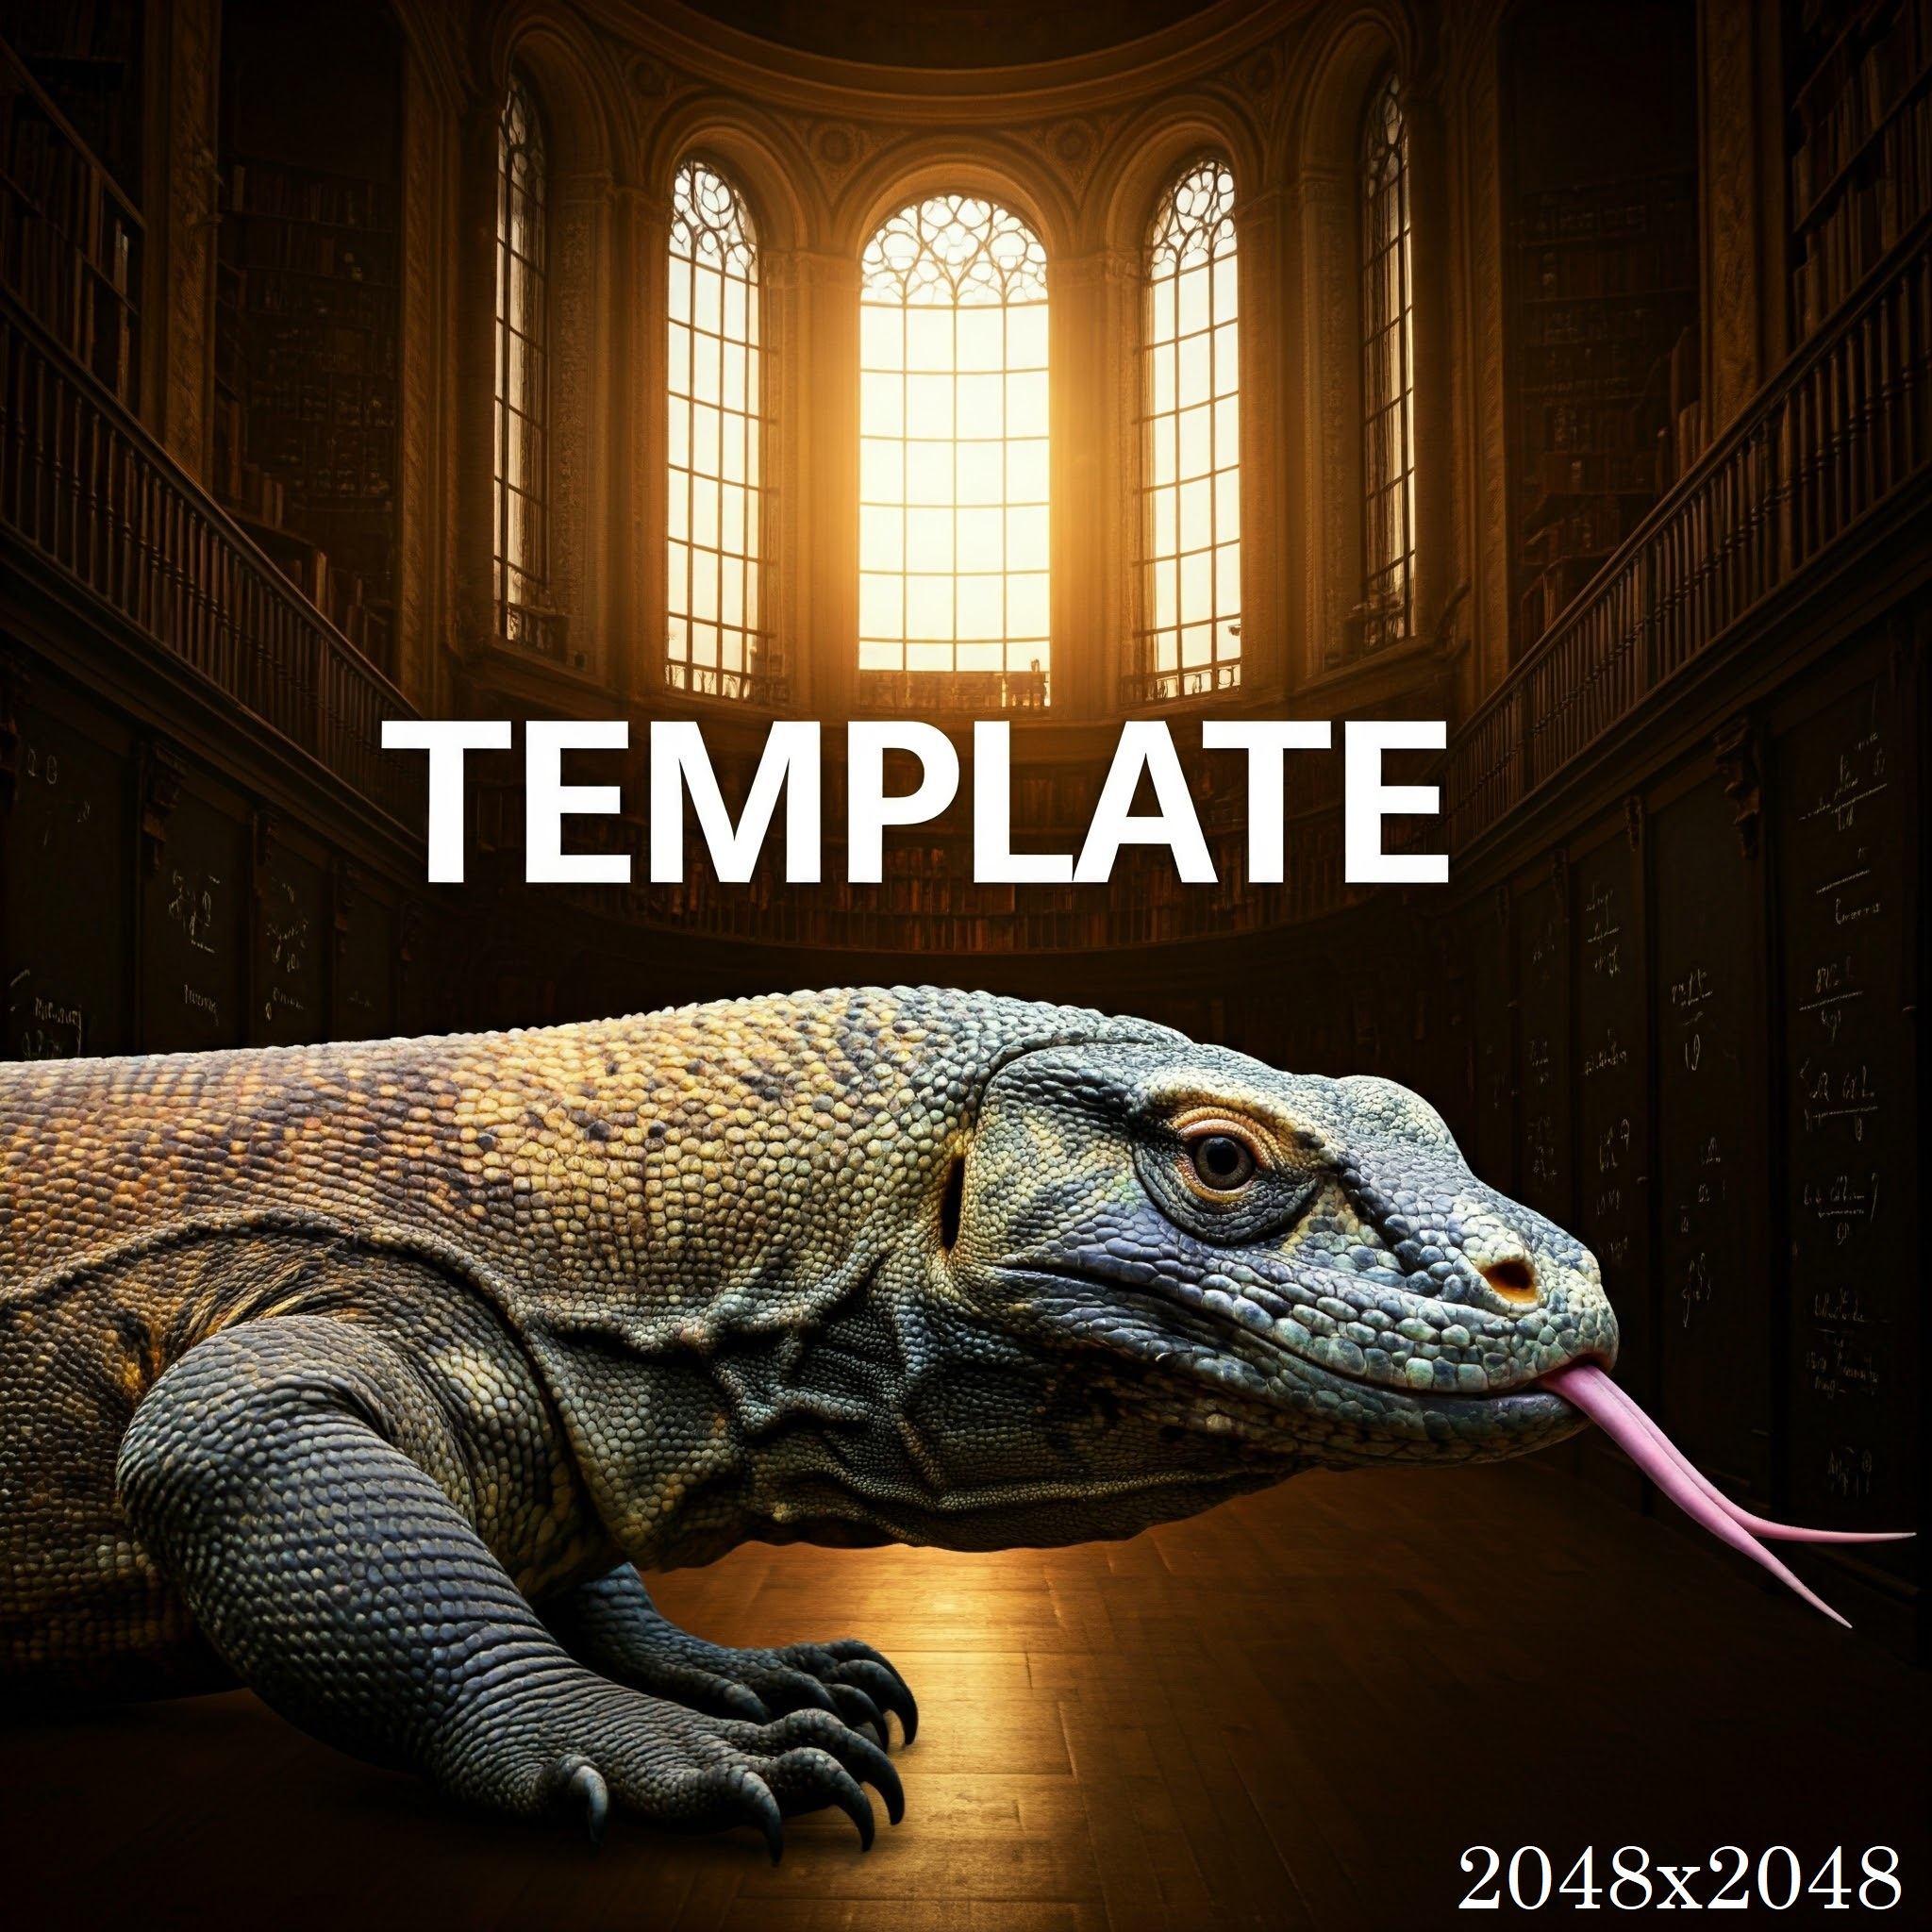
\includegraphics[width=1\textwidth ]{images/copertina.jpg}
    }
\end{figure}
\vfill 
\centering 
\includegraphics[width=0.4\textwidth ]{../../preamble/Stemma_sapienza.png} \acc
\centering \Large \color{sapienza}Facoltà di Ingegneria dell'Informazione,
Informatica e Statistica\\
Dipartimento di Informatica
\end{titlepage}

%===================FINE COPERTINA======================%
\newpage
\pagecolor{cartaRiciclata}%\setmainfont{Algerian}
\Large
Questo documento è distribuito sotto la licenza 
\color{blue}\href{https://www.gnu.org/licenses/fdl-1.3.txt}{GNU}\color{black},  
è un resoconto degli appunti (eventualmente integrati con libri di testo) tratti dalle lezioni del corso di \jobname
\hphantom{a}per la laurea 
triennale in Informatica. Se dovessi notare errori, ti prego di segnalarmeli.
\newpage %\setmainfont{Times New Roman}
\normalsize
\tableofcontents 
\newpage

%==================FOOTER e HEADER=======================%
\fancyhf{}
\fancyhead[L]{\nouppercase{\leftmark}}
\fancyhead[R]{Sezione \thesection}
\fancyfoot[C]{\thepage}
\fancyfoot[L]{Appunti di \jobname}
\fancyfoot[R]{ Marco Casu}
%\fancyfoot[R]{\setmainfont{Palace Script MT}\huge Marco Casu \setmainfont{Times New Roman}}
%==================FOOTER e HEADER=======================%

%Ricorda del comando \flowerLine per separare le sottosezioni. Le sezioni si separano nelle diverse pagine

%==================INIZIO======================%




\chapter{Meccanica Degli Omozigoti}
\section{Introduzione}
\lipsum[1]
\subsection{Risvolti storici}
\lipsum[2]\acc 
\teo{del costo unitario}ogni costo è unitario, ogni uomo ha un anima, le seguente è vera
$$ a(x)\ne b(x)\iff a\sim e^{sin(x^2)}$$
\dimo{}Segue dalla proposizione atomica decuplicante $\blacksquare$\acc \lipsum[2]\acc
\prop{}Il cane è blu \flowerLine 
\section{La nascita della Fisica Moderna}
\lipsum[1] \ref{fig:birds} \lipsum[2]
\begin{figure}[h!]
    \centering
    \begin{tikzpicture}
        \begin{axis}[
            axis lines = left,
            xlabel = \(x\),
            ylabel = {\(f(x)\)},
        ]
        %Below the red parabola is defined
        \addplot [
            domain=-5:5, 
            samples=200, 
            color=red,
        ]
        {sin(deg(x))*cos(deg(e^x))};
        \addlegendentry{\(\sin(x)\cdot \cos(e^x)\)}
        \end{axis}
        \end{tikzpicture}
    \caption{limite}
    \label{fig:birds}
\end{figure}\acc
\lipsum[3]
\subsection{Carico e Scarico}
\lipsum[2]
\eqImportante{$\displaystyle M(k)=\iint_{\R^3}\sum_{n = 1}^{k}x^2y^4z^{e^-\pi}dxdydz$}
\lipsum[1]\acc  
Questi sono gli appunti di \jobname.
\flowerLine 
\section{Cani}
\lipsum[2]
\begin{figure}[h!]
    \centering
    \begin{tikzpicture}
        \begin{axis}[
            axis lines = left,
            xlabel = \(x\),
            ylabel = {\(f(x)\)},
        ]
        %Below the red parabola is defined
        \addplot [
            domain=-10:10, 
            samples=200, 
            color=blue,
        ]
        {x*((1/x)*cos(deg(e^(sin(deg(x))))))};
        \end{axis}
        \end{tikzpicture}
\end{figure}\acc
\lipsum[3]
\newpage
\chapter{Disossamenti}
\lipsum[1]\flowerLine 
\section{Costanza e Porte}
\lipsum[2]
$$ \iint _\Omega F = kk$$\lipsum[3] 
\end{document}
